\documentclass[10pt,a4paper]{article}

\usepackage[a4paper, top=0.9cm, bottom=0.9cm, left=1cm, right=1cm]{geometry}
\usepackage{graphicx}
\usepackage{float}
\usepackage{amsmath}
\usepackage{amssymb}
\usepackage{xcolor}
\usepackage{mdframed}
\usepackage{parskip}
\usepackage{enumitem}
\usepackage{titlesec}
\usepackage{booktabs}
\usepackage{array}
\usepackage{tikz}
\usetikzlibrary{arrows.meta, positioning}
\usepackage[T1]{fontenc}

\graphicspath{{../../reference/Network_extracted/figures/Lecture2/}}

% ── Colours ────────────────────────────────────────────────────────────────
\definecolor{keyblue}{RGB}{30, 80, 160}
\definecolor{keybluebg}{RGB}{220, 235, 255}
\definecolor{noteorange}{RGB}{200, 100, 0}
\definecolor{noteorangebg}{RGB}{255, 240, 215}
\definecolor{warnred}{RGB}{180, 30, 30}
\definecolor{warnredbg}{RGB}{255, 220, 220}
\definecolor{defgreen}{RGB}{20, 110, 50}
\definecolor{defgreenbg}{RGB}{215, 245, 225}
\definecolor{headernavy}{RGB}{25, 35, 90}

\newmdenv[linecolor=keyblue,backgroundcolor=keybluebg,linewidth=1.5pt,
  leftline=true,rightline=false,topline=false,bottomline=false,
  innerleftmargin=7pt,innerrightmargin=6pt,
  innertopmargin=3pt,innerbottommargin=3pt,
  skipabove=3pt,skipbelow=3pt]{keybox}

\newmdenv[linecolor=noteorange,backgroundcolor=noteorangebg,linewidth=1.5pt,
  leftline=true,rightline=false,topline=false,bottomline=false,
  innerleftmargin=7pt,innerrightmargin=6pt,
  innertopmargin=3pt,innerbottommargin=3pt,
  skipabove=3pt,skipbelow=3pt]{notebox}

\newmdenv[linecolor=defgreen,backgroundcolor=defgreenbg,linewidth=1.5pt,
  leftline=true,rightline=false,topline=false,bottomline=false,
  innerleftmargin=7pt,innerrightmargin=6pt,
  innertopmargin=3pt,innerbottommargin=3pt,
  skipabove=3pt,skipbelow=3pt]{defbox}

\newmdenv[linecolor=warnred,backgroundcolor=warnredbg,linewidth=1.5pt,
  leftline=true,rightline=false,topline=false,bottomline=false,
  innerleftmargin=7pt,innerrightmargin=6pt,
  innertopmargin=3pt,innerbottommargin=3pt,
  skipabove=3pt,skipbelow=3pt]{warnbox}

\titleformat{\section}[block]{\normalsize\bfseries\color{headernavy}}{}{0pt}{}
  [\vspace{1pt}\rule{\linewidth}{0.6pt}\vspace{2pt}]
\titleformat{\subsection}[block]{\small\bfseries\color{keyblue}}{}{0pt}{}
\titlespacing*{\section}{0pt}{5pt}{2pt}
\titlespacing*{\subsection}{0pt}{3pt}{1pt}

\setlist{nosep, topsep=1pt, itemsep=1pt, leftmargin=1.3em}
\parskip=2pt
\parindent=0pt

% ===========================================================================
\begin{document}
% ===========================================================================

\begin{center}
  {\large\bfseries\color{headernavy} Q2 \textemdash{} CAN Bus \& FlexRay}\\[1pt]
  {\small MM2 $\cdot$ Hans-Peter Schwefel}
\end{center}
\vspace{1pt}\hrule height 1pt\vspace{5pt}

We look at two fieldbus protocols used in embedded/automotive systems:
% ===========================================================================
\section*{1\quad Fieldbus Overview}
% ===========================================================================

\begin{keybox}
\textbf{Fieldbus} = single closed network operating mainly at \textbf{OSI layers 1\&2}
(sometimes also layer 7). \\ nodes share one bus.
\end{keybox}

% ===========================================================================
\section*{2\quad CAN Bus --- Physical Layer \& Arbitration}
% ===========================================================================
All nodes connect to a shared \textbf{differential pair} bus (CAN\_H and CAN\_L), terminated at each end with a 124\,$\Omega$ resistor to prevent signal reflections. Bits are encoded as voltage differences between the two lines.

% ── Left col: TikZ bus topology + voltage ─────────────────────────────────
\begin{minipage}[t]{0.46\textwidth}
\small\textit{Bus topology (differential pair, shared):}\\[4pt]
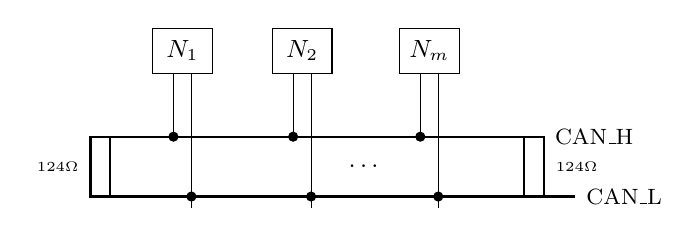
\begin{tikzpicture}[>=Stealth, font=\small, scale=0.95]
  % ── Two horizontal bus lines ──────────────────────────────────
  \draw[thick] (0.15, 0.5) -- (5.65, 0.5);
  \draw[thick] (0.15,-0.3) -- (6.35,-0.3);   % CAN_L extends right past resistor
  \node[right, font=\footnotesize] at (5.95, 0.5)  {CAN\_H};
  \node[right, font=\footnotesize] at (6.37,-0.3)  {CAN\_L};
  % ── Left terminator resistor (square box) ─────────────────────
  \draw[thick] (-0.13,-0.3) rectangle (0.13,0.5);
  \node[left, font=\tiny] at (-0.16,0.1) {124$\Omega$};
  % ── Right terminator resistor (square box) ────────────────────
  \draw[thick] (5.67,-0.3) rectangle (5.93,0.5);
  \node[right, font=\tiny] at (5.96,0.1) {124$\Omega$};
  % ── Nodes: two separate wires, left→CAN_H, right→CAN_L ───────
  \foreach \x/\lbl in {1.1/N_1, 2.7/N_2, 4.4/N_m} {
    % node box above
    \draw (\x-0.40, 1.35) rectangle (\x+0.40, 1.95);
    \node[font=\small] at (\x, 1.65) {$\lbl$};
    % left wire: connects to CAN_H only
    \draw (\x-0.12, 1.35) -- (\x-0.12, 0.5);
    \draw[fill=black] (\x-0.12, 0.5) circle (0.06);
    % right wire: connects to CAN_L only (offset right, extends past line)
    \draw (\x+0.12, 1.35) -- (\x+0.12, -0.45);
    \draw[fill=black] (\x+0.12, -0.3) circle (0.06);
  }
  % ellipsis between N_2 and N_m
  \node at (3.55, 0.1) {\small\ldots};
\end{tikzpicture}
\vspace{3pt}
\begin{notebox}
\textbf{Why differential pair?} Noise hits both wires equally --- receiver reads the \emph{difference}, so common-mode interference cancels out. Crucial in noisy automotive environments.
\end{notebox}
\end{minipage}\hfill
% ── Right col: arbitration rules + example ────────────────────────────────
\begin{minipage}[t]{0.50\textwidth}
\small\textit{Voltage levels (recessive = 2.5\,V both, dominant = spread):}\\[3pt]
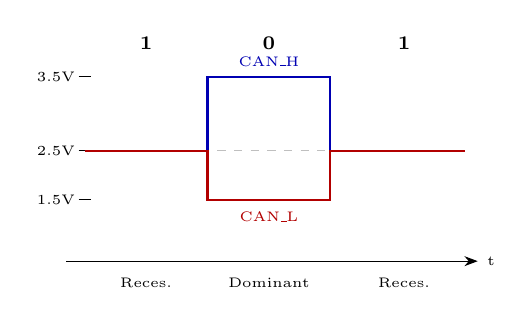
\begin{tikzpicture}[>=Stealth, font=\tiny, scale=0.78]
  \draw[->] (-0.3,0) -- (6.4,0) node[right]{t};
  \foreach \y/\lbl in {1/1.5, 1.8/2.5, 3/3.5} {
    \draw (-0.1,\y) -- (0.1,\y); \node[left] at (0,\y) {\lbl V};
  }
  \draw[dashed,gray!50] (0,1.8) -- (6.2,1.8);
  % Bit labels on top: 1, 0, 1
  \node[font=\scriptsize\bfseries] at (1.0, 3.55) {1};
  \node[font=\scriptsize\bfseries] at (3.0, 3.55) {0};
  \node[font=\scriptsize\bfseries] at (5.2, 3.55) {1};
  % CAN_H
  \draw[blue!70!black, thick]
    (0,1.8) -- (2,1.8) -- (2,3) -- (4,3) -- (4,1.8) -- (6.2,1.8);
  \node[blue!70!black] at (3.0,3.25) {CAN\_H};
  % CAN_L
  \draw[red!70!black, thick]
    (0,1.8) -- (2,1.8) -- (2,1) -- (4,1) -- (4,1.8) -- (6.2,1.8);
  \node[red!70!black] at (3.0,0.72) {CAN\_L};
  % Region labels
  \node at (1.0,-0.35) {Reces.};
  \node at (3.0,-0.35) {Dominant};
  \node at (5.2,-0.35) {Reces.};
\end{tikzpicture}
\vspace{3pt}
\begin{defbox}
\textbf{Recessive (1):} both lines at 2.5\,V\\
\textbf{Dominant (0):} CAN\_H$\uparrow$ 3.5\,V, CAN\_L$\downarrow$ 1.5\,V\\
Dominant \textbf{always overwrites} recessive.
\end{defbox}
\end{minipage}
% ===========================================================================
\section*{2b\quad CAN ID \& Arbitration}
% ===========================================================================
Since dominant (0) always overwrites recessive (1), priority is determined by the CAN ID: the node with the \textbf{lowest ID wins} the bus automatically.\\
\begin{minipage}[t]{0.46\textwidth}
\begin{keybox}
\textbf{Arbitration --- lowest ID wins:}
\begin{itemize}
  \item Only Tx when \textbf{bus is idle}
  \item All nodes send CAN ID simultaneously
  \item Read back bus while sending; if read $\neq$ sent $\Rightarrow$ \textbf{stop}
  \item Dominant (0) overwrites recessive (1)
  \item Messages have IDs $\Rightarrow$ diff.\ priority msgs
  \item \textbf{Error detection}: error $\Rightarrow$ retransmit
\end{itemize}
\end{keybox}
\end{minipage}\hfill
% ── Right col: arbitration rules + example ────────────────────────────────
\begin{minipage}[t]{0.50\textwidth}

\vspace{4pt}
\textbf{Example} --- 3 nodes transmit simultaneously:

\vspace{2pt}
\begin{tabular}{@{}l|cccc|l@{}}
\toprule
      & b1 & b2 & b3 & b4 & Result \\\midrule
N$_1$ & 0  & 0  & 0  & 0  & \textcolor{defgreen}{\textbf{Sends}} \\
N$_2$ & 0  & 0  & 1  &    & \textcolor{warnred}{Stops (b3)} \\
N$_3$ & 0  & 0  & 0  & 1  & \textcolor{warnred}{Stops (b4)} \\\bottomrule
\end{tabular}

\vspace{4pt}
\begin{notebox}
\small\textit{Relates to Q4 (Network Calculus):} CAN/FlexRay
traffic can be modelled as arrival curves --- used to
compute worst-case delay bounds for safety-critical messages.
\end{notebox}
\end{minipage}
% ===========================================================================
\section*{Note \quad CAN Bit Stuffing, Bit Timing \& RTT (Don't say only for remember)}
% ===========================================================================
\begin{notebox}
\begin{minipage}[c]{0.4\textwidth}
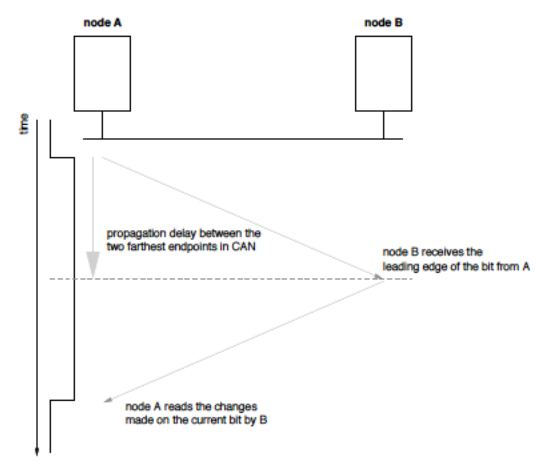
\includegraphics[width=\linewidth]{progationtiming.png}
\end{minipage}\hfill
\begin{minipage}[c]{0.43\textwidth}
\begin{warnbox}
\textbf{RTT constraint:} A$\to$B$\to$A must fit within 1 bit time so arbitration works. Limits max bus length.\\[3pt]
\small 1\,Mbit/s $\Rightarrow$ 1\,µs $\Rightarrow$ $\approx$40\,m\\
125\,kbit/s $\Rightarrow$ $\approx$500\,m
\end{warnbox}
\begin{keybox}
\textbf{Bit stuffing:} after 5 identical bits, CAN inserts an opposite \emph{stuff bit}.\\[2pt]
\textbf{Why:} guarantees transitions for receiver clock recovery.\\[2pt]
\textbf{Bit timing:} each bit = time quanta (TQ). Sample point programmable within the bit --- must account for propagation delay (RTT $\leq$ 1 bit time).
\end{keybox}
\end{minipage}
  
\end{notebox}


\clearpage
% ===========================================================================
\section*{3\quad FlexRay --- Communication Cycle}
% ===========================================================================
Unlike CAN's event-driven arbitration, FlexRay is \textbf{time-triggered}: every node follows a fixed repeating \textbf{communication cycle} split into 4 segments.
\begin{itemize}
  \item \textsc{The cycle length is determined by the \textbf{shortest periodic requirement} in the system --- all timing is pre-planned, giving deterministic worst-case guarantees.
}
\end{itemize}

\vspace{4pt}
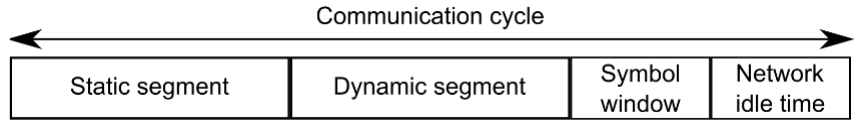
\includegraphics[width=0.88\linewidth]{flexraycommunicationcycle.png}

\vspace{4pt}

\begin{minipage}[t]{0.48\textwidth}
\subsection*{Static Segment (always starts at action point)}
\begin{itemize}
  \item Divided into \textbf{equal-size slots}, node always transmits in its slot
  \item \# slots per node depends on node bandwidth use
  \item Worst-case delay: \textbf{at most 1 cycle}
\end{itemize}

\subsection*{Symbol Window}
Special bit pattern transmitted, e.g.\ \textbf{waking up a node}.
\end{minipage}\hfill
\begin{minipage}[t]{0.49\textwidth}
\subsection*{Dynamic Segment (priority on node ID)}
\begin{itemize}
  \item Always same \# mini-slots but \textbf{different dynamic slot counter}
  \item Always fills \textbf{1 mini-slot} even when not transmitting
  \item Each node has \textbf{pLatestTx} (latest possible Tx time) --- if not reached in time $\Rightarrow$ wait next cycle
\end{itemize}

\subsection*{Network Idle Time}
Corrects \textbf{microtick} adjustments to align with \textbf{macrotick} perfectly (clock sync).
\end{minipage}

\vspace{4pt}
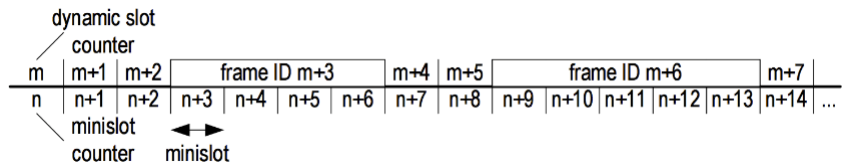
\includegraphics[width=0.88\linewidth]{minislotting.png}

\section{Rest Extra Here Under}
% ===========================================================================
\section*{4\quad CAN vs FlexRay --- Use Case Comparison}
% ===========================================================================

\vspace{2pt}
\begin{tabular}{@{}lll@{}}
\toprule
& \textbf{CAN} & \textbf{FlexRay} \\\midrule
Cost        & Cheap                    & Expensive \\
Throughput  & Lower rate               & Higher rate \\
Traffic     & Bursty / event-driven    & Periodic + bursty \\
Timing      & Not life-critical        & Exact, deterministic \\
Reliability & ---                      & 2-channel redundancy \\
Use case    & Body electronics, sensors & Chassis, safety-critical (X-by-wire) \\
\bottomrule
\end{tabular}

\begin{notebox}
\small \textbf{Key distinction:} CAN uses \emph{arbitration} (event-driven, non-deterministic worst-case);
FlexRay uses \emph{TDMA} (time-triggered, guaranteed slots, deterministic worst-case delay).
\end{notebox}
% ===========================================================================
\section*{6\quad FlexRay --- Timing Hierarchy \& Clock Sync}
% ===========================================================================

\begin{minipage}[c]{0.52\textwidth}
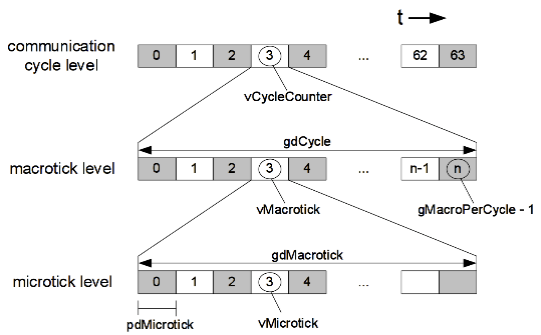
\includegraphics[width=\linewidth]{flexrayTimingHier.png}
\end{minipage}\hfill
\begin{minipage}[c]{0.45\textwidth}
\begin{defbox}
\textbf{Microtick} = smallest hardware clock unit (node-local oscillator).\\[2pt]
\textbf{Macrotick} = agreed global time unit, built from microticks.\\[2pt]
\textbf{NIT} at end of each cycle corrects drift: nodes adjust how many microticks per macrotick so all stay aligned.
\end{defbox}
\vspace{3pt}
\begin{notebox}
\small CAN has \textbf{no global clock} --- sync per-bit via edge detection. FlexRay NIT maintains a \textbf{fault-tolerant distributed clock} $\Rightarrow$ deterministic slot timing.
\end{notebox}
\end{minipage}

\vspace{4pt}


\end{document}
